% Author: Dr. Matthias Jung, DL9MJ
% Year: 2021

\usetikzlibrary{calc, positioning}
\usepackage{pgfplotstable}
\usepackage{amsmath}
\usepackage{unicode-math}
\setmathfont{Fira Math}
\setmathfont[range=up]{Roboto}
\setmathfont[range=it]{Roboto-Italic}
\setmathfont[range=\int]{Fira Math}
\usepackage[euler]{textgreek}

\begin{document}
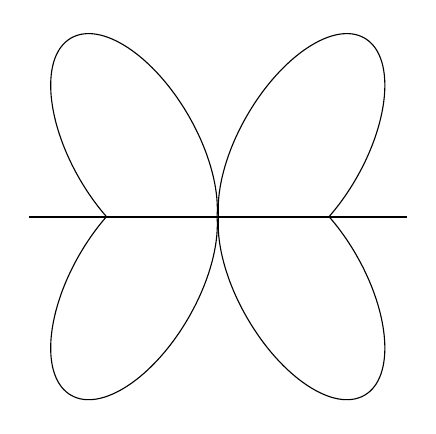
\begin{tikzpicture}
\begin{scope}[shift={(7,0)},scale=0.8]
\foreach\i/\j in {1/1,1/-1,-1/1,-1/-1}
{
  \begin{scope}[x=\i cm,y=\j cm]
    \clip (0,0) rectangle (3,3);
    \draw[rotate=60*\i*\j] (1.62,-0.6) ellipse (2cm and 1cm);
  \end{scope}
 }
\draw[thick] (-3,0) -- (3,0);
\end{scope}
\end{tikzpicture}
\end{document}
